\chapter{Literature Review}
\label{chap:litreview}
	In order to understand the need for a clinical method of detecting deep tissue injuries, the full scope and current state of the issue must be explored. To this end, the current state of the literature regarding deep tissue injuries, how they form, what factors characterize them, and how they are currently treated is explored here. In order to relate this disease to the detection modality proposed in this work, the mechanics and history of ultrasound elastography are also explored and related back to the problem at hand. The major gaps in the current literature regarding the use of ultrasound elastography for detecting and monitoring deep tissue injuries are presented as these gaps are what this work attempts to begin to fill.

	\section{Deep Tissue Injuries}
		Pressure ulcers, commonly referred to as ``bedsores'', are an extraordinarily large problem facing the health care system today. At least \SI{11}[\$]{billion} is spent in the United States of America alone treating approximately 500,000 injuries annually \cite{beckrich99,russo08} while only a minute fraction of that is spent toward pressure ulcer research \cite{zanca03}. Compared to hospital stays for all other conditions, patients with at least a secondary diagnosis of a pressure ulcer were more often discharged to a long-term care facility and more likely resulted in death \cite{russo08}. These injuries place an extremely significant burden on the people who suffer from them---pressure ulcers were found to have a profound impact on people's lives including: altering their physical, social, and financial status; changing their body image; losing independence and control; and subjecting them to the grieving process \cite{langemo00,baharestani94}. \note[KH]{I already mentioned this in the introduction, verbatim. Where should it go?}These debilitating wounds are often suffered by people with limited mobility such as those undergoing lengthy surgical procedures, the elderly, and those with spinal cord injuries (SCI) \cite{allman95}---approximately \SI{80}{\percent} of people with spinal cord injuries (SCI) will develop at least one pressure ulcer during their lifetime \cite{salzberg96} and approximately \SI{19}{\percent} of elderly patients in long-term care facilities will develop one \cite{freitas11}. Pressure ulcers exist throughout the entire health-care system and are often formed when undergoing hospitalization \cite{aronovitch99}. These injuries have a tendency to become chronic, non-healing wounds and many patients die from complications related to them \cite{jaul10}. Further, patients who have developed at least one pressure ulcer in their life are at a significantly greater risk of developing a second \cite{niazi97}. Pressure ulcers and deep tissue injuries generally form at the bone-muscle interface deep in the tissue \cite{kanno09} with approximately \SI{64}{\percent} occurring over the ischial tuberosities, trochanter, or sacrum \cite{garber03}. In general, these injuries are characterized by a some manner of tissue loss through necrosis of the tissue, though there is currently some debate on the exact nature of these wounds as well as the accuracy of the clinical descriptions attributed to them by the National Pressure Ulcer Advisory Panel (NPUAP).

		The NPUAP defines pressure ulcers as a ``localized injury to the skin and / or underlying tissue usually over a bony prominence, as a result of pressure, or pressure in combination with shear and / or friction'' and are generally staged according to a tiered system of increasing damage \cite{npuap07}. The various stages are depicted in Fig. \ref{fig:npuap-staging} and described as follows:

		\begin{figure*}[!t]
			\centering
			\subfloat[Normal tissue]{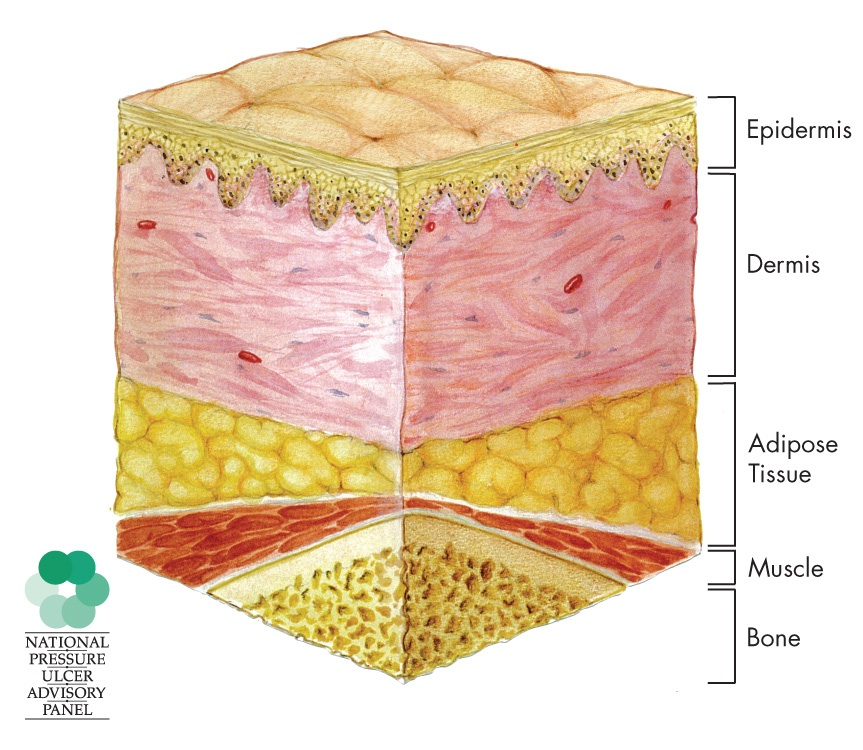
\includegraphics[width=0.3\textwidth]{images/npuap/normal.png}\label{fig:npuap-normal}}

			\subfloat[Stage I]{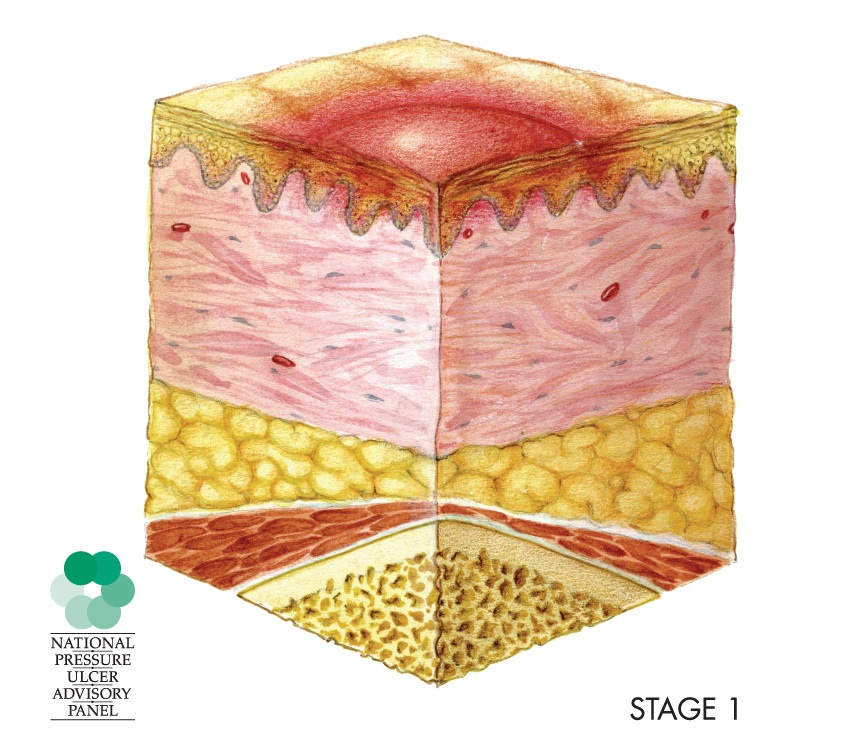
\includegraphics[width=0.3\textwidth]{images/npuap/stage1.png}\label{fig:npuap-stage1}}
			\subfloat[Stage II]{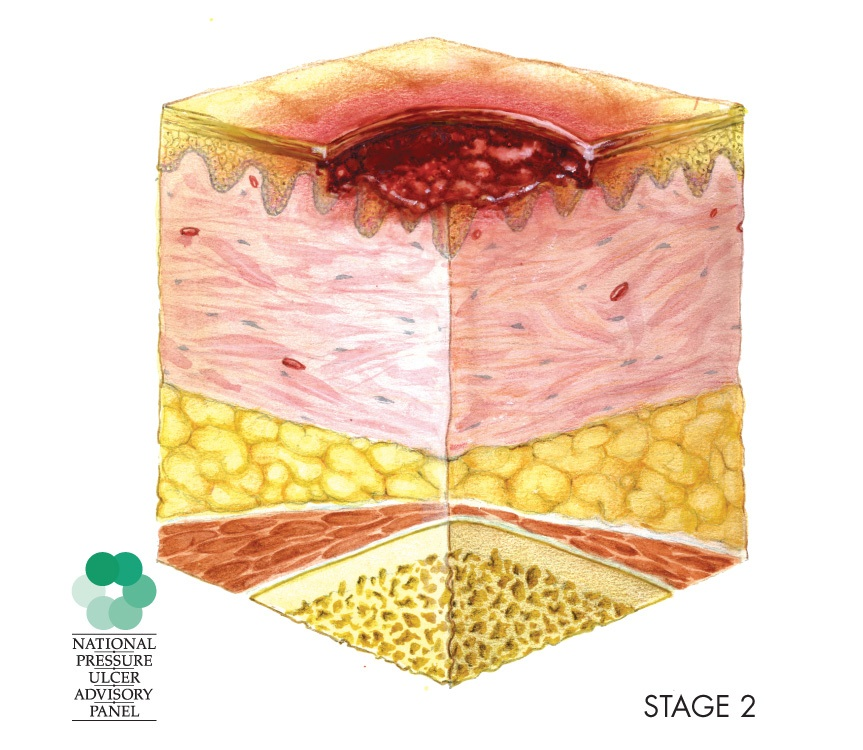
\includegraphics[width=0.3\textwidth]{images/npuap/stage2.png}\label{fig:npuap-stage2}}
			\subfloat[Stage III]{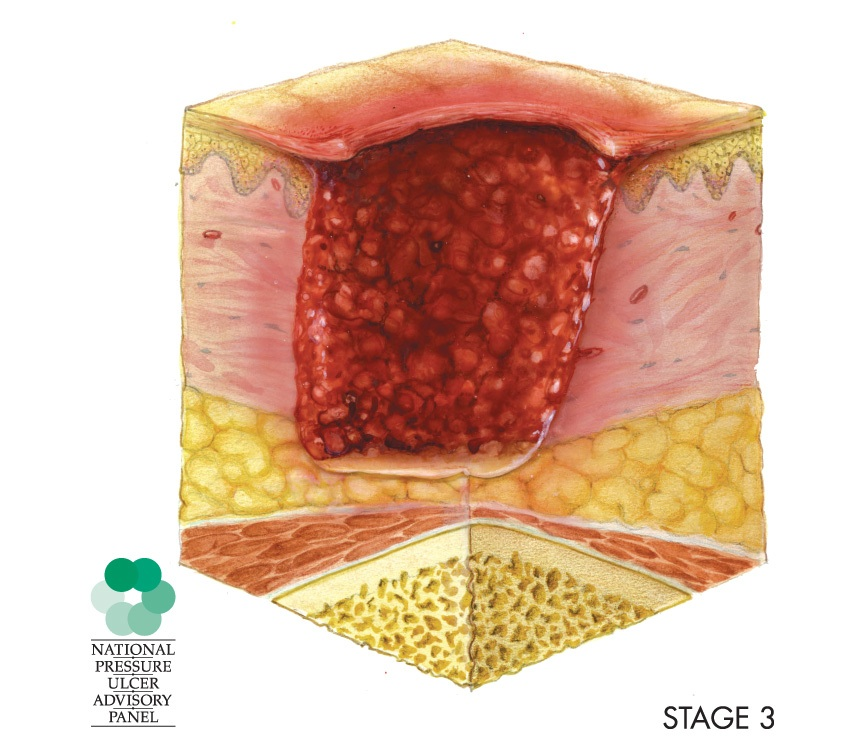
\includegraphics[width=0.3\textwidth]{images/npuap/stage3.png}\label{fig:npuap-stage3}}

			\subfloat[Stage IV]{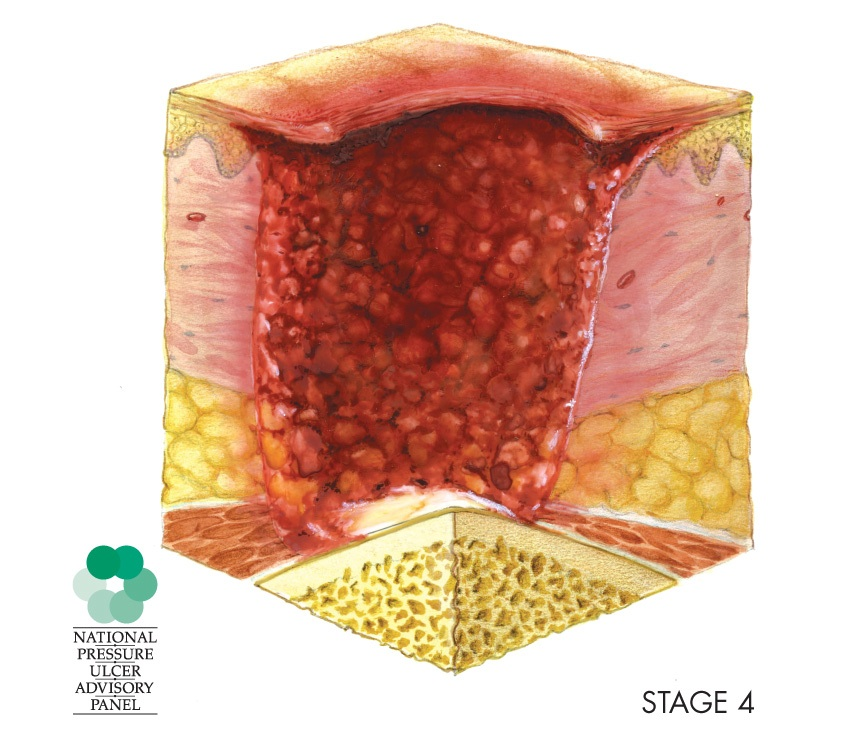
\includegraphics[width=0.3\textwidth]{images/npuap/stage4.png}\label{fig:npuap-stage4}}
			\subfloat[Unstageable]{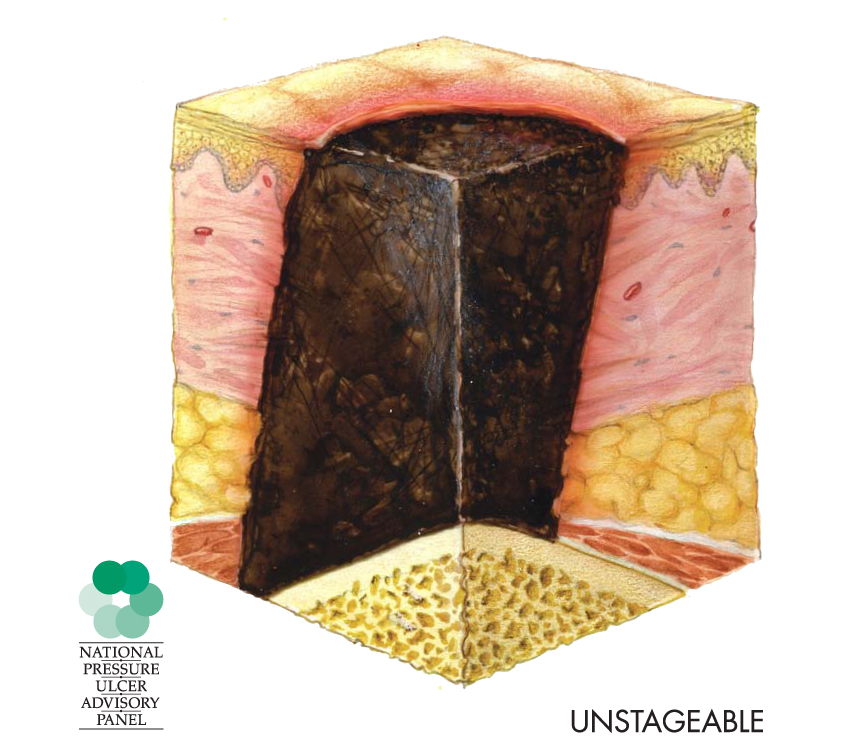
\includegraphics[width=0.3\textwidth]{images/npuap/unstageable.png}\label{fig:npuap-unstageable}}
			\subfloat[Suspected DTI]{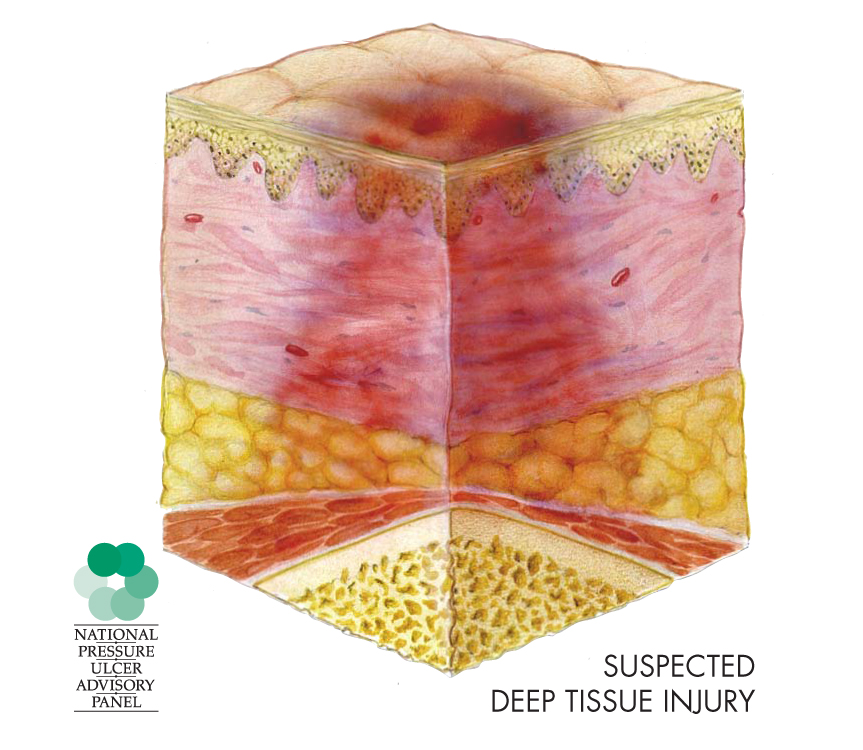
\includegraphics[width=0.3\textwidth]{images/npuap/suspectedDTI.png}\label{fig:npuap-dti}}
			\caption[NPUAUP pressure ulcer staging guidelines]{The NPUAP staging guideline illustrations of the various stages / severities of pressure ulcers.}
			\label{fig:npuap-staging}
		\end{figure*}

		\begin{description}
			\item[Suspected Deep Tissue Injury] \hfill \\
				Purple or maroon localized area of discoloured intact skin or blood-filled blister due to damage of underlying soft tissue from pressure and / or shear. The area may be preceded by tissue that is painful, firm, mushy, boggy, warmer or cooler as compared to adjacent tissue.
			\item[Stage I] \hfill \\
				Intact skin with non-blanchable redness of a localized area usually over a bony prominence. Darkly pigmented skin may not have visible blanching; its colour may differ from the surrounding area.
			\item[Stage II] \hfill \\
				Partial thickness loss of dermis presenting as a shallow open ulcer with a red pink wound bed, without slough. May also present as an intact or open / ruptured serum-filled blister.
			\item[Stage III] \hfill \\
				Full thickness tissue loss. Subcutaneous fat may be visible but bone, tendon or muscle are not exposed. Slough may be present but does not obscure the depth of tissue loss. \emph{May} include undermining and tunnelling.
			\item[Stage IV] \hfill \\
				Full thickness tissue loss with exposed bone, tendon or muscle. Slough or eschar may be present on some parts of the wound bed. Often include undermining and tunnelling.
			\item[Unstageable] \hfill \\
				Full thickness tissue loss in which the base of the ulcer is covered by slough (yellow, tan, grey, green, or brown) and / or eschar (tan, brown or black) in the wound bed.
		\end{description}

		The NPUAP's definitions of pressure ulcers come from clinical experiences with them and are largely based on the ulcer's appearance after they have formed and do not necessarily reflect the true aetiological factors that lead to these conditions. For example, a significant body of literature scientifically describes deep tissue injuries as being much more insidious than a ``localized area of discoloured intact skin'' and suggests that many Stage III and IV pressure ulcers are actually advanced deep tissue injuries rather than advanced Stage I or II ulcers \cite{gefen09}. This chasm between the clinically accepted and scientifically observed definitions of deep tissue injuries is likely due to the lack of any clinical detection ability \cite{campbell10}. What is agreed upon is that deep tissue injuries are a major problem and more needs to be done to facilitate preventing and treating them \cite{black11,maklebust05} and one of the largest hurdles to preventing and treating DTI is the lack of any substantial early detection ability \cite{gunningberg08,milne09}.

		\subsection{Aetiology and Histology}
			\label{sec:litreview-aetiology}
			Deep tissue injuries are thought to occur through the combinatory effects of three distinct but related mechanisms: ischemia, insufficient lymph drainage, and cell deformation. Ischemia is a condition where the blood supply to tissue has been cut off, rendering the tissue unable to function appropriately. Insufficient lymph drainage refers to how waste products may accumulate in tissue when the lymph vessels that normally carry them away become occluded. Cell deformation occurs when mechanical strains are imparted upon the tissue, causing excessive deformation in not only the extracellular matrix, but in the cells as well. Taken together, the presence of these factors has been shown to greatly increase the risk of developing a deep tissue injury \cite{stekelenburg08}.

			For quite some time, ischemia was regarded as the chief acute risk factor for developing late-stage pressure ulcers \cite{witkowski82,dinsdale74,kosiak61}. Although studies have shown that healthy tissue is able to survive complete ischemia for approximately 4 hours before severe necrosis set in \cite{labbe87,strock69}, deep tissue injuries are clinically found when loading times are substantially less than this \cite{aronovitch99,bliss99}. The model of ischemic damage alone could not account for the rate of late-stage pressure ulcers that we were witnessed.

			Once it was realized that ischemia alone could not be the culprit behind deep tissue injury formation, ischemia-induced reperfusion injury became implicated in the formation of DTI \cite{Ytrehus95,Blaisdell02,tsuji05}. An ischemia-induced reperfusion injury is caused when blood is allowed to flow back into a region of tissue that was previously ischemic. While seeming somewhat contrary to its expected effect, the restoration of circulation results in a swelling and inflammatory effect which causes extensive microvascular damage \cite{Blaisdell02}. The effect of reperfusion was confirmed when comparing pure ischemic conditions in tissue to a cycle of ischemic-reperfused conditions over the same period of time, where it was found that significantly greater damage was caused by repeated loading-unloading rather than simple constant loading \cite{tsuji05,salcido94}. While ischemia-reperfusion injuries provide a more complete explanation about the formation of deep tissue injuries, they still do not account for those injuries acquired under constant pressure over short time periods.

			In order for cells to function in a healthy manner, the waste they produce must be constantly carried off and processed via the lymphatic system and its series of lymph vessels that perfuse tissue. If the magnitude of pressure applied to tissue reaches a threshold level, the pressure occludes the lymph vessels and lymphatic drainage ceases \cite{miller81}. Once lymphatic drainage ceases, cell waste accumulates in the tissue and is thought to initiate necrosis in the cells \cite{krouskop78,reddy81,braden87}. Since this model of damage relates to occlusion of vessels, inhibited lymphatic drainage may be categorized as an ischemic risk factor.

			In order to account for deep tissue injuries that form over short time periods, a model of cell deformation leading to necrosis has more recently been proposed \cite{landsman95,bouten01,wang05}. It has constantly been observed that tissue regions which eventually form deep tissue injuries exhibit signs of locally increased strains \cite{stekelenburg06,ceelen08,linderganz08,portnoy09,solis12-03}, with greater degrees of deformation correlating to greater degrees of damage. To account for these results, it has been proposed that excessively deforming strains applied to cells over extended periods of time can alter the permeability of the cell's plasma membranes, leading to an overall reduced cell viability \cite{slomka12}. Further, it has been shown both in finite-element models and experimentally that the stiffness of soft tissue and the corresponding strains that are developed within them are closely related \cite{loerakker13,gefen05,linderganz09,nagel09}. Not only does the amount of deformation depend on the stiffness of tissue, but the stiffness of tissue was found to correlate to the level of deep tissue injury damage seen in the resulting histology \cite{gefen04} with immediate 1.6-fold to 3.3-fold stiffening of the tissue occurring immediately after injury \cite{gefen05,linderganz04}. Further, the stiffness of tissue severely drops below that of healthy tissue when it begins to decompose \cite{gefen05,dimaio01}, leading to a relationship between injury progression and stiffness as shown in Fig. \ref{fig:stiffness-time-relation} (adapted from \cite{gefen09}).

			\begin{figure}[!t]
				\centering
					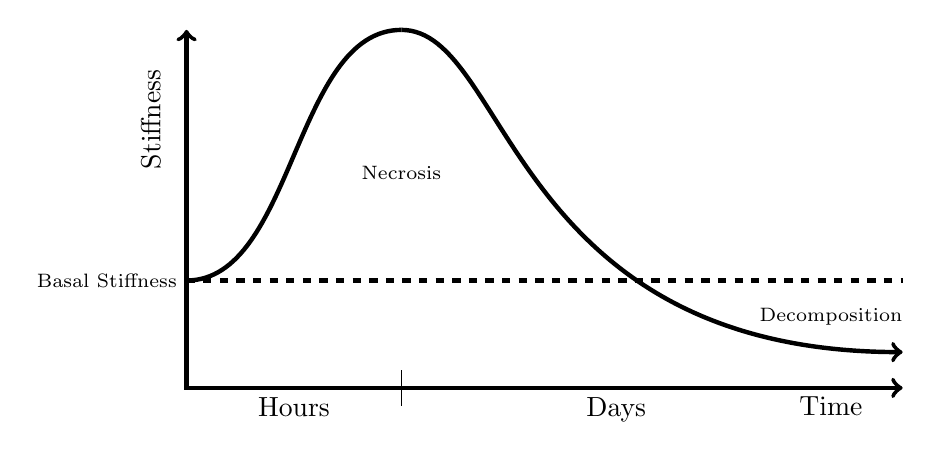
\begin{tikzpicture}[x=0.75\textwidth,y=0.375\textwidth]
						% basal stiffness
						\draw[ultra thick, dashed]
						(0, 0.3) -- (1, 0.3);

						% stiffness curve
						\draw[ultra thick] plot[smooth, tension=1] (0, 0.3) .. controls(0.15, 0.3) and (0.15, 1) .. (0.3, 1);
						\draw[ultra thick, ->] plot[smooth, tension=1] (0.3, 1) .. controls(0.45, 1) and (0.45, 0.1) .. (1, 0.1);

						% axes
						\draw[ultra thick, <->] (0, 1) -- (0, 0) -- (1, 0);

						% time tick
						\draw (0.3, -0.05) -- (0.3, 0.05);

						\node[below] at (0.15, 0) {Hours};
						\node[below] at (0.6, 0) {Days};
						\node[rotate=90] at (-0.05, 0.75) {Stiffness};
						\node[left] at (0, 0.3) {\scriptsize Basal Stiffness};
						\node at (0.3, 0.6) {\scriptsize Necrosis};
						\node at (0.9, 0.2) {\scriptsize Decomposition};
						\node at (0.9, -0.05) {Time};
					\end{tikzpicture}
				\caption[Schematic representation of the time course of tissue stiffness changes in a deep tissue injury site.]{Schematic representation of the time course of tissue stiffness changes in a deep tissue injury site. The estimate for the time-course for local rigor mortis was obtained from animal model studies \cite{portnoy08} and the estimate for the time-course for tissue decomposition was obtained from the forensic literature \cite{dimaio01}. (Adapted from Gefen \cite{gefen09})}
				\label{fig:stiffness-time-relation}
			\end{figure}

			There have been many models of deep tissue injury formation throughout the years, each relating to different mechanisms, though all relating to mechanical stress of the tissue, either through vessel occlusion or direct cellular strain. The truth is most likely a combination of these effects, with cell deformation dominating the damage on shorter time scales with increased applied pressure and vessel occlusion type injuries dominating on longer time scales \cite{stekelenburg08}. In order to further investigate the etiology of PU and DTI, a combination of experimental and numerical studies has been suggested to provide better fundamental knowledge besides existing clinical experience \cite{bouten03}. There is also significant evidence in the literature that suggests that the current NPUAP definitions of PU and DTI are unacceptable and not based on scientific evidence and that updating the clinical definitions to better reflect what exists in the literature is crucial to increasing the success of diagnosis and treatment of PU and DTI \cite{gefen09,campbell10}.

			\comment{
				Other possible papers to cite:
					\cite{ceelen08-8}: Computational model that shows how cells that die under compression decrease in stiffness.
					\cite{gefen07-9}: Review of knowledge of DTI aetiology, and why the NPUAP definition is shitty
					\cite{linderganz06}: Greatest strain occurs deep in the tissue, not at the surface
					\cite{then09}: Material information for examining soft tissue deformation
					\cite{vanNierop10}: Diffusion of water affected only by tissue temperature, not deformation
					\cite{salcido94}: Lesions occur deep in tissue rather than at the surface
					\cite{gefen07}: Sitting posture greatly changes the damage that occurs in PU
					\cite{oomens10}: Interface pressure is not a good measure of tissue health, but rather internal strains are
			}

		\subsection{Detection}
			As previously mentioned, there is a lack of means for detecting the early onset of deep tissue injuries in a clinical setting \cite{gunningberg08,milne09}. Currently, when attempting to detect and diagnose a deep tissue injury or pressure ulcer, clinicians generally rely upon a risk-factor scale for patients rather than actually detecting a lesion. Popular risk assessment tools include the Norton, Braden, and Risk Assessment Pressure Sore scales which each attempt to predict the formation of a pressure ulcer in a patient given their scores in a series of relatively subjective variables such as ``general physical condition'' and ``mental state'' \cite{norton63,braden94,lindgren02}. Aside from these main risk-assessment scales, multiple other scales have been proposed for specific populations such as SCI patients \cite{salzberg96} and oncology patients \cite{fromantin11}. While these tools assist health-care practitioners to manage their limited resources with regards to patient care, at best they only provide guesses as to who will develop pressure ulcers or not. The sensitivity---the ability to correctly diagnose an existing condition---of these techniques ranges from approximately \SI{42}{\percent} -- \SI{87}{\percent} while the specificity---the ability to correctly determine that no condition is present---ranges from \SI{57}{\percent} -- \SI{88}{\percent} \cite{kallman14}. Other studies have shown that nurses have great difficulty detecting and diagnosing suspected deep tissue injuries given the current frameworks they are provided \cite{lee13}, while physicians are even worse \cite{levine12}. While these scales are ``better than nothing'' at diagnosing patients with pressure ulcers, they are far from ideal and are simply not capable of actually diagnosing this disease---for that, a quantifiable detection technology is required.

			In pressure ulcer research it is common to evaluate the extent of deep tissue injury formation through the use of $\mathrm{T}_2^*$-weighted MRI \cite{loerakker11,stekelenburg06,solis12-03}. $\mathrm{T}_2^*$-weighted MRI is able to detect deep tissue injury by investigating tissue oxygenation as a proxy for detecting the lack of cellular activity due to necrosis. Although this technique is well suited for research purposes, it is simply not viable for detecting and monitoring the progression of DTI in the large population of at-risk patients. At the time of writing, MRI scans can easily cost upwards of \SI{1000}[\$]{} and take over an hour to complete \note[KH]{Citation needed!}. Further, patients with implants such as pacemakers and who make up a large proportion of the at-risk population cannot undergo MRI scans due to the large magnetic forces involved and / or the need to relocate from their hospital bed to the stationary MRI machine. Of the alternative diagnostic imaging modalities that currently exist, ultrasound provides the most promise due to it's ability to non-invasively interrogate tissues in a mobile and cost-effective manner.

			B-mode ultrasound scans involve the sonographic interrogation of a tissue's acoustic properties by transmitting sound waves on the order of multiple \si{MHz} and ``listening'' to the waves as they are reflected in tissue. B-mode ultrasound imaging has been used to identify hypo-echoic regions in sub-epidermal tissue related to DTI \cite{andersen08,aoi08,kanno09}, however the results from these studies are somewhat unclear and require a degree of interpretation of the results. After combining thermographic techniques with b-mode imaging results, it may be possible to increase the accuracy of early deep tissue injury detection \cite{higashino12}. As a more reliable alternative, ultrasound elastography---a sonographic technique for interrogating tissue strains rather than acoustic properties---has been proposed as a possible tool for clinical diagnosis of DTI \cite{gehin06,gefen09,gefen13}. Some exploratory studies have successfully used this technique to quantify deep tissue injury formation not only numerically, but in {PVA}-cryogel phantoms as well as in a rat model \cite{deprez07,deprez11}. While these studies show promise, they are only the beginning for the adoption of ultrasound elastography as a viable clinical detection modality for deep tissue injuries.

			Recently, another possible avenue for DTI detection has arisen which lies in the biochemical markers present in a patient's blood or urine. Rhabdomyolysis refers to the process when myoglobin proteins from damaged skeletal muscle enter the bloodstream due to a breakdown of muscle fibres in the body. Although this condition may be caused by numerous factors such as hyperthermia, ingestion of various drugs, alcohol abuse, toxins, autoimmune disease, or physical damage \cite{beetham00,sauret02}, it may also be an indicator of formative DTI in at-risk patients who do not present with any of the aforementioned risk factors. Myoglobin proteins present in the blood get filtered in the kidneys and as such can present in the urine, turning it tea-brown \cite{bagley07}.

			With the many avenues of DTI detection currently being explored and utilized, it is most likely that a combination of all the techniques will provide the most utility. For example, upon hospital admission or with a reasonably high risk assessment score, a patient may be given a blood test which confirms the presence of a forming injury or not. Patients with forming injuries may then be scanned using ultrasound technology to locate and quantify the injury. That patient may then receive more targeted care, of which the effectiveness may be continually monitored using both blood and ultrasound tests. It is expected that the targeted care that this approach would provide would increase patient health and well-being while at the same time decreasing the overall load on the health-care system.

		\subsection{Prevention and Treatment}
			The current state of deep tissue injury treatment and prevention largely reflects the lack of a quantifiable detection modality. One of the most commonly used preventions is called ``turning'' whereby patients are repositioned in their beds or wheelchairs such that individual regions of tissue are intermittently relieved of pressure. Although commonly implemented in health care settings, turning has repeatedly been found to be inadequate at reducing the incidence of pressure ulcers \cite{vanderwee07,rich11}. A more technological means of reducing the mechanical loads on tissue lies in support surface design \cite{krouskop86}. Unlike turning, pressure-redistribution foam mattresses have repeatedly shown their ability to reduce the incidence of pressure ulcers in a cost-effective manner \cite{pham11,rafter11}. Despite the effectiveness of these surfaces however, the overall prevalence rate of pressure has not changed significantly, suggesting that appropriate preventions are not being utilized in health-care settings \cite{maklebust05}.

			An emerging technology in the realm of pressure ulcer prevention is intermittent electrical stimulation (IES). IES is the process by which electrical impulses are utilized to activate muscle fibres and contract the muscle. IES has been found to not only increase the oxygenation in deep tissue \cite{gyawali11}, but also significantly reduce the damage caused from excessive loading \cite{solis13}. While still being developed, IES may prove to be an extremely effective preventative therapy for DTI.

			While various technologies exist or are in development for preventing pressure ulcers, little is available to treat them when they occur. Generally, pressure ulcer treatment involves optimizing regional blood flow, managing underlying illnesses, and providing adequate nutrition \cite{jaul10}. If a pressure ulcer has become chronic, treatment switches to controlling the symptoms and preventing complications \cite{jaul10}. Negative pressure wound therapy is a process by which a slight vacuum is applied to the open wound for several weeks and has shown some success in reducing the severity of late-stage pressure ulcers \cite{greer13}. Surgical techniques such a debriding may also be used in an attempt to remove necrotic tissue from the wound and prevent it from growing any larger \cite{longe86,brem02}. Skin-flap surgery is often used on chronic ulcers in an attempt to protect the wound bed \cite{biglari14}.

			When various prevention and treatment paradigms are implemented, the incidence of hospital-acquired pressure ulcers may decrease dramatically \cite{bales11,thompson11,carson11}. However, one of the key required areas of improvement is in the detection and monitoring of pressure ulcers \cite{milne09}---without the ability to continually monitor a wound, the true effectiveness of any given therapies is indeterminate.

	\section{Ultrasound Elastography}
		%\lipsum[1]

		\subsection{Quasi-Static Ultrasound Elastography}
			\comment{
				papers:
					\cite{osanai11}
			}

		\subsection{Acoustic Radiation Force Impulse Imaging}

		\subsection{Shear Wave Speed Quantification}

	\section{Numerical Characterization / Finite-Element Modelling}
		%\lipsum[1]

	\section{Conclusion}
		%\lipsum[1]

	\cleardoublepage

	\phantomsection

	\addcontentsline{toc}{section}{References}
	%\bibliographystyle{IEEEtran}
	%\renewcommand{\bibliography}[1]{}
	%\bibliography{references}
	\bibcomplete{references}
	\printbibliography[heading=subbibliography]